\subsection{Ca sử dụng xem ảnh theo địa điểm}

Sau khi cập nhật vị trí cho ảnh, người dùng có thể xem danh sách ảnh đã chụp tại một địa điểm cụ thể. Hệ thống sẽ tự động lấy vị trí hiện tại của người dùng (nếu được cấp quyền) và hiển thị danh sách ảnh trên bản đồ. Người dùng có thể bấm vào ảnh trong danh sách để xem vị trí chi tiết của ảnh trên bản đồ. Với yêu cầu là trước đó, hệ thống đã hoàn thành phân loại các nhóm địa điểm ảnh.

Mô tả chi tiết cho ca sử dụng xem ảnh theo địa điểm được thể hiện ở Bảng \ref{tab:view-image-location-usecase} dưới đây. Kèm theo là Bảng \ref{tab:view-image-location-usecase-activity} về biểu đồ hoạt động, quan hệ và Hình \ref{fig:3-3-14-sequence-diagram} về biểu đồ tuần tự của ca sử dụng này. 

\noindent 
\begin{table}[H]
\centering
\caption{Mô tả chi tiết ca sử dụng xem ảnh theo địa điểm}
\label{tab:view-image-location-usecase}
\begin{tabularx}{\linewidth}{| l | X |} 
\hline 
\textbf{Mô tả} & Người dùng xem danh sách ảnh được chụp tại 1 địa điểm. \\
\hline 
\textbf{Luồng cơ bản} & 1. Người dùng bấm vào nhóm địa điểm muốn xem danh sách ảnh chụp tại nơi đó. \newline
                       2. Hệ thống điều hướng đến trang danh sách ảnh của địa điểm. \newline
                       3. Hệ thống lấy thông tin danh sách ảnh chụp tại địa điểm và nhóm theo ngày. \newline
                       4. Hệ thống hiển thị hộp thoại cấp quyền thông tin vị trí hiện tại. \newline
                       5. Người dùng cấp quyền truy cập vị trí hiện tại. \newline
                       6. Hệ thống hiển thị danh sách ảnh chụp trên bản đồ. \\
\hline
\textbf{Luồng thay thế} & - Người dùng không cấp quyền truy cập vị trí. \newline
                          - Hệ thống không lấy được dữ liệu ảnh của địa điểm. \\
\hline
\textbf{Tiền điều kiện} & - Người dùng đã đăng nhập vào hệ thống. \newline
                          - Có ít nhất 1 bức ảnh đã được cập nhật vị trí chụp ảnh. \\
\hline
\textbf{Hậu điều kiện} & - Người dùng có thể bấm vào ảnh trong danh sách để xem vị trí chi tiết của ảnh trên bản đồ. \\
\hline 
\textbf{Yêu cầu phi chức năng} & - Hệ thống lấy dữ liệu ảnh của địa điểm không quá 1s. \newline
                           - Hệ thống lấy được dữ liệu hiện tại vị trí người dùng (nếu được cấp quyền). \\
\hline 
\end{tabularx}
\end{table}

\noindent 
\begin{table}[H]
\centering
\caption{Biểu đồ hoạt động và quan hệ ca sử dụng xem ảnh theo địa điểm}
\label{tab:view-image-location-usecase-activity}
\begin{tabular}{| c | c |}
    \hline
    \textbf{Biểu đồ hoạt động} & \textbf{Quan hệ} \\ 
    \hline
    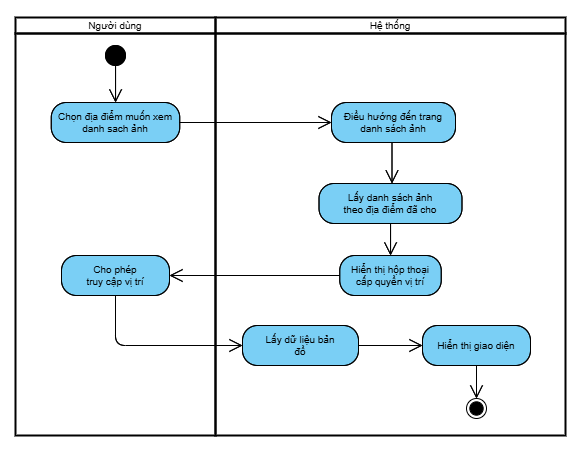
\includegraphics[width=0.6\linewidth]{figures/c3/3-3-14-activity-diagram.png} 
    &  
    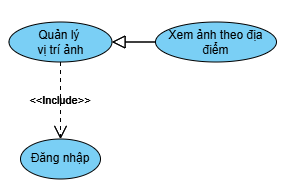
\includegraphics[width=0.35\linewidth]{figures/c3/3-3-14-relationship.png} \\ 
    \hline
\end{tabular}
\end{table}

\begin{figure}[H]
    \centering  
    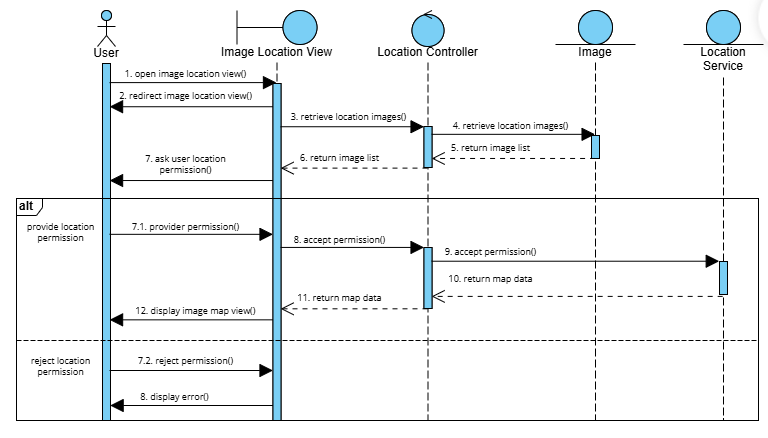
\includegraphics[width=1.1\textwidth]{figures/c3/3-3-14-sequence-diagram.png}
    \caption{Biểu đồ tuần tự ca sử dụng xem ảnh theo địa điểm.}
    \label{fig:3-3-14-sequence-diagram}
\end{figure}